\documentclass[xcolor=table]{beamer}

\mode<presentation> {
  \usetheme{CambridgeUS}
}
\usecolortheme{seahorse}
\setbeamertemplate{navigation symbols}{}

\usepackage{graphicx} % Allows including images
\usepackage{booktabs} % Allows the use of \toprule, \midrule and \bottomrule in tables

\usepackage[utf8]{inputenc}
\usepackage[T2A]{fontenc}
\usepackage[english,russian]{babel}
\usepackage{listings}
\usepackage{xcolor}
\usepackage{caption}
\usepackage{stmaryrd}



\usepackage{biblatex}

\bibliography{main2.bib}

\newcommand{\citepres}[1]{{\it \citetitle{#1}}, \citeauthor{#1}, \citeyear{#1}}

\renewcommand{\footnotesize}{\tiny}

\title[Университет ИТМО]{Применение метода суперкомпиляции для специализации реляционных программ}

\author{Мария Куклина, M4236}
\institute[ITMO]
{
Университет ИТМО\\ 

Научный руководитель: Близнец Иван Александрович\\
Научный консультант: Вербицкая Екатерина Андреевна \\

2020
\medskip
}
\date{}


\begin{document}

\begin{frame}
\titlepage
\end{frame}

%
% TODO: footnote цвет более серый

%%%%%%%%%%%%%%%%%%%%%%%%%%%%%%%%%%%%%%%%%%%%%%%%%%%
%
%
%%%%%%%%%%%%%%%%%%%%%%%%%%%%%%%%%%%%%%%%%%%%%%%%%%%
\begin{frame}{Реляционное программирование}
\begin{block}{Определение}
    Вид декларативного программирования, в котором программы представляются как набор отношений между аргументами.
\end{block}
\begin{block}{Пример}
  Пример {\it запросов} для отношения умножения $\text{mul}^o \subseteq \text{Int} \times \text{Int} \times \text{Int}$:
  \begin{itemize}
    \item $\texttt{mul}^o(\texttt{2, 2, 4})$ --- проверка корректности отношения.
    \item $\texttt{mul}^o(\texttt{2, 2, C})$ --- поиск всех \texttt{С}, таких что \texttt{2 * 2 = C}.
    \item $\texttt{mul}^o(\texttt{A, 1, 4})$ --- поиск всех \texttt{A}, таких что \texttt{A * 1 = 1}.
    \item $\texttt{mul}^o(\texttt{A, B, C})$ --- поиск всех троек \texttt{A, B, С}, таких что \texttt{A * B = C}.
  \end{itemize}
\end{block}
\end{frame}
%%%%%%%%%%%%%%%%%%%%%%%%%%%%%%%%%%%%%%%%%%%%%%%%%%%
%
%
%%%%%%%%%%%%%%%%%%%%%%%%%%%%%%%%%%%%%%%%%%%%%%%%%%%
\begin{frame}{miniKanren}
  \begin{block}{}
    Встраиваемый предметно-ориентированный язык реляционного программирования\footnotemark.
    % Сказать про логическое программирование в ограничениях
  \end{block}\footnotetext{\citepres{byrdMK}}

  {\bf Применение}
  \begin{itemize}
  % \item Замена тяжеловесной подсистемы Prolog для ряда задач.
  \item Легковесная логическая подсистема проекта.
  \item Поиск лечения редких генетических заболеваний в точной медицине\footnote{\citepres{medMK}}.
  \item Генерация программ по спецификации входов и выходов на основе \emph{реляционного интерпретатора}.
  \item Порождение решения задач поиска по решению задачи распознавания\footnote{\citepres{lozov}}.
  \end{itemize}
\end{frame}
%%%%%%%%%%%%%%%%%%%%%%%%%%%%%%%%%%%%%%%%%%%%%%%%%%%
%
%
%%%%%%%%%%%%%%%%%%%%%%%%%%%%%%%%%%%%%%%%%%%%%%%%%%%
\begin{frame}{Постановка проблемы}

\begin{itemize}
\item Сложные алгоритмы в miniKanren работают медленно.
\item
  % Многие отношения на деле являются функциональными, из-за чего запуск в ``обратном'' направлении очень неэффективен.\\
  Поиск входов по выходам отношения работает значительно медленнее, чем ``прямой'' запуск.\\
  {\bf Примеры}
  \begin{itemize}
  \item Программы, порождённые инструментом по трансляции из функционального языка в miniKanren\footnote{\citepres{trconv}}.
  \item Порождение решения задач поиска.
  \end{itemize}
\end{itemize}
\end{frame}
%%%%%%%%%%%%%%%%%%%%%%%%%%%%%%%%%%%%%%%%%%%%%%%%%%%
%
%%%%%%%%%%%%%%%%%%%%%%%%%%%%%%%%%%%%%%%%%%%%%%%%%%%
\begin{frame}{Специализация}
\begin{block}{Определение}
Автоматизированная техника оптимизации программ, при которой из программы удаляются
избыточные вычисления, зависимые от частично известного входа\footnotemark.
\end{block}\footnotetext{\citepres{jones}}

\begin{itemize}
\item Частичная дедукция --- класс методов специализации для логический языков, в частности, для Prolog.\footnote{\citepres{advanced}}
\item Специализация miniKanren на основе \emph{конъюнктивной частичной дедукции (CPD)}\footnote{\citepres{lozov}}.
\begin{itemize}
\item Сложна в поддержке, даёт нестабильные результаты.
\item Однако предоставляет библиотеку для построения специализаторов.
\end{itemize}
\end{itemize}
\end{frame}
%%%%%%%%%%%%%%%%%%%%%%%%%%%%%%%%%%%%%%%%%%%%%%%%%%%
%
%%%%%%%%%%%%%%%%%%%%%%%%%%%%%%%%%%%%%%%%%%%%%%%%%%%
\begin{frame}{Суперкомпиляция}

\begin{block}{Определение}
Техника автоматической трансформации и анализа программ, при которой
программа символьно исполняется с сохранением истории вычислений, на основе
которой принимаются решения о трансформации и оптимизации.
\end{block}

\begin{itemize}
\item Суперкомпиляторы применяются во основном для функциональных языков\footnote{\citepres{scPos}}.
\item % Суперкомпиляция показывает хорошие результаты при специализации.
      Суперкомпиляция позволяет достичь не более чем линейного ускорения\footnote{\citepres{scompRevisited}}
\item Полуавтоматическая суперкомпиляция для Prolog\footnote{\citepres{apropos}}.
\item Теоретические доводы для автоматической суперкомпиляции для $\text{Prolog}^{\text{9}}$.
\end{itemize}

\end{frame}
%%%%%%%%%%%%%%%%%%%%%%%%%%%%%%%%%%%%%%%%%%%%%%%%%%%
%
%
%%%%%%%%%%%%%%%%%%%%%%%%%%%%%%%%%%%%%%%%%%%%%%%%%%%
\begin{frame}{Цели и задачи}
\begin{block}{Цель}
Улучшение результатов специализации реляционных программ путём применения метода суперкомпиляции.
\end{block}
%%%%%%%%%%%%%%%%%%%%%%%%%%%%%%%%%%%%%%%%%%%%%%%%%%%
%
%
%%%%%%%%%%%%%%%%%%%%%%%%%%%%%%%%%%%%%%%%%%%%%%%%%%%
\begin{block}{Задачи}
\begin{itemize}
\item Реализовать базовый суперкомпилятор для miniKanren.
\item Рассмотреть возможные методы улучшения получившегося суперкомпилятора.
\item Протестировать результаты и сравнить их c результатами CPD и c оригинальными программами.
\end{itemize}
\end{block}
\end{frame}


%%%%%%%%%%%%%%%%%%%%%%%%%%%%%%%%%%%%%%%%%%%%%%%%%%%
%
%
%%%%%%%%%%%%%%%%%%%%%%%%%%%%%%%%%%%%%%%%%%%%%%%%%%%
% \begin{frame}{$\mu$Kanren}
% \begin{block}{Определение}
% Минимальное подмножество miniKanren, содержащее в себе только основные операции языка:
% конъюнкция, дизъюнкция,
% унификация, введение свежей переменной и вызов реляционного отношения.\\
% \end{block}
% \begin{itemize}
% \item Программа на $\mu$Kanren представляет собой логическую формулу, атомы которой --- это либо унификация двух термов, либо вызов отношения.
% \item Не содержит операторов miniKanren c эффектами. 
% \item Библиотека для специализации работает с $\mu$Kanren\footnote{\url{https://github.com/kajigor/uKanren_transformations}}.
% \end{itemize}
% \end{frame}

%%%%%%%%%%%%%%%%%%%%%%%%%%%%%%%%%%%%%%%%%%%%%%%%%%%
%
%
%%%%%%%%%%%%%%%%%%%%%%%%%%%%%%%%%%%%%%%%%%%%%%%%%%%
\begin{frame}{Суперкомпиляция для miniKanren}

\begin{figure}[h!]
\center
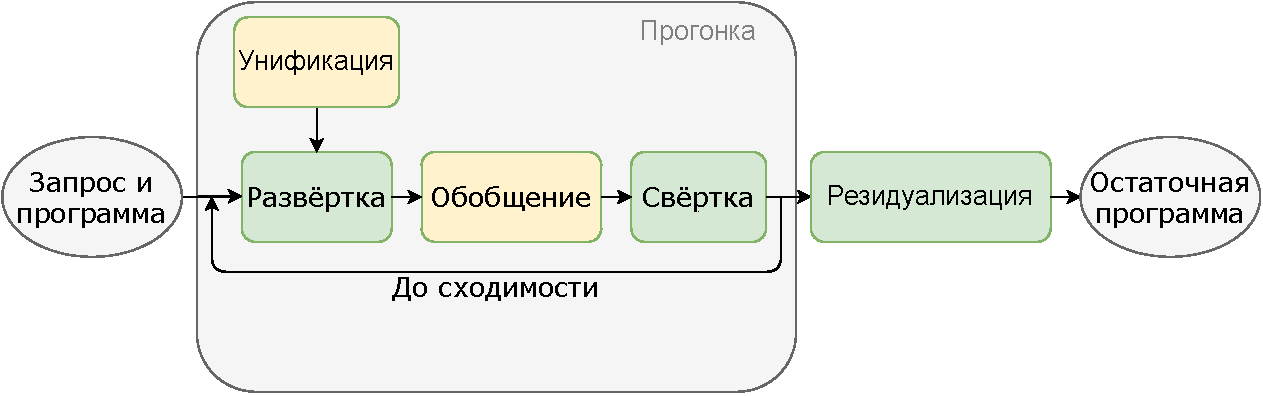
\includegraphics[scale=0.55]{scompflow.pdf}
\caption{
    Схема алгоритма суперкомпиляции\\
}
\label{fig:scomp}
\end{figure}
{\footnotesize
\begin{tabular}{l}

\includegraphics[scale=0.4]{orange.pdf} --- библиотека по специализации miniKanren c дополнениями\\

\includegraphics[scale=0.4]{green.pdf} --- собственная разработка
\end{tabular}
}


%В процессе суперкомпиляции строится корневой ориентированный граф, описывающий историю символьного исполнения,
%из которого извлекается \emph{остаточная} программа --- специализированная версия исходной.

\end{frame}

\begin{frame}{Особенности шага развёртки для miniKanren}
\begin{block}{}
{\bf Развёртка} определяет шаг символьного вычисления в суперкомпиляторе,
на котором порождается множество возможных состояний программы.
\end{block}
\vspace{0.5cm}
\begin{block}
{\bf Значимые отличия}
\begin{itemize}
\item Несколько возможных шагов вычисления.
\item Допускается переупорядочивание элементов выражения.
% \item Реляционность предполагает, что методы специализации логических
%\item Допускает больше возможностей для суперкомпиляции, чем другие языки.
\end{itemize}
\end{block}
\end{frame}

\begin{frame}{Результаты задачи}
\begin{itemize}
\item Реализован базовый алгоритм суперкомпиляции.
\begin{itemize}
\item Развёртка рассматривает все возможные состояния.
\item Используемый алгоритм обобщения основан на алгоритме для конъюнктивной частичной дедукции,
      для которого доказана терминируемость.
% \item Стратегия вычисления соответствует семантике языка.
\end{itemize}
\item Разработан и реализован алгоритм построения оптимизированной программы по графу суперкомпиляции.
\end{itemize}
\end{frame}

\begin{frame}{Улучшение суперкомпиляции для miniKanren}
\begin{block}{Проблемы}
\begin{itemize}
%\item Свёртка только на родителей: повторные символьные вычисления.
\item Повторение символьных вычислений из-за стратегии свёртки.
%Решается кэшированием.
% \item Обобщение: слишком много вычислений перед свёрткой.
\item Классическое использование обобщения может приводить к избыточным вычислениям.
\begin{itemize}
\item Существует техника обобщения, описанная в статьях\footnotemark.
\item Придумана специфичная для miniKanren техника обощения.
\end{itemize}

\item Тривиальная стратегия вычисления порождает слишком много ветвей исполнения.
%Решение: исследовать способы реализации шага прогонки.
\item В используемой реализации miniKanren нет способа эффективно сообщить, что можно прервать вычисление.
%Решение: расширить язык оператором неравенства из miniKanren.
\end{itemize}
\end{block}
\footnotetext{\citepres{scPos}}
%\begin{block}{Дополнительные техники}
%\begin{itemize}
%\item Модификация обобщения, позволяющая добиться улучшения качества специализации.
%\end{itemize}
%\end{block}
\end{frame}

\begin{frame}{Результаты задачи}
\begin{itemize}
\item Применены подходы по улучшению алгоритма суперкомпиляции.
\begin{itemize}
\item Добавлено кэширование.
\item Реализованы модификации обобщения.
\item Проанализированы и реализованы допустимые стратегии вычисления.
\end{itemize}
\item Расширение библиотеки для специализации неравенствами.
\item Расширение суперкомпилятора, при котором учитывается
      ``негативная'' информация.
\end{itemize}
\end{frame}

%%%%%%%%%%%%%%%%%%%%%%%%%%%%%%%%%%%%%%%%%%%%%%%%%%%
%
%%%%%%%%%%%%%%%%%%%%%%%%%%%%%%%%%%%%%%%%%%%%%%%%%%%
\begin{frame}{Тестирование}

\begin{description}[leftmargin=!]
\item[Реализация miniKanren:] проект OCanren\footnote{\url{https://github.com/JetBrains-Research/OCanren}}\\
\item[Реализация CPD для miniKanren:] проект uKanren\_transformations\footnote{\url{https://github.com/kajigor/uKanren_transformations/}}
\item[Реализация CPD для Prolog:] проект ECCE\footnote{\url{https://github.com/leuschel/ecce}}
\item[Платформа:] Intel Core i5-6200U CPU, 2.30GHz, DDR4, 12GiB.
\end{description}
{\bf Сценарий тестирования:}
\begin{enumerate}
\item Суперкомпиляция тестовой программы.
\item Трансляция остаточной программы в OCanren.
\item Замер времени исполенения.
\item Сравнение времени исполнения с оригинальной программой и реализациями CPD.
\end{enumerate}
\end{frame}

%%%%%%%%%%%%%%%%%%%%%%%%%%%%%%%%%%%%%%%%%%%%%%%%%%%
%
%%%%%%%%%%%%%%%%%%%%%%%%%%%%%%%%%%%%%%%%%%%%%%%%%%%
\begin{frame}{Тестирование}
{\small Программы для тестирования}
\begin{description}
\item[sort]Алгоритм реляционной сортировки.\\
      % Запрос: $\text{sort}^o$ xs ys.
      Запрос : сортировка случайного списка длины 50
\item[isPath] Проверка принадлежности пути графу.\\
      % Запрос: $\text{isPath}^o$ p g true.
      Запрос: поиск  произвольного пути длины 10, принадлежащих графу c 21 вершиной и 50 рёбрами.
\item[logint] Реляционный интерпретатор формул логики высказываний.\\
      Запрос: поиск 1000 истинных формул в данной подстановке.
      % Запрос: $\text{logint}^o$ s q true.
\item[lam] Реляционный интерпретатор лямбда-выражений.\\
      % Запрос: $\text{lam}^o$ q q.
      Запрос: поиск n термов, сводящихся к указаной форме.
% \item Реляционный алгоритм вывода типов для просто типизированного лямбда-исчисления.
%\item[a] Реляционный интерпретатор подмножества Scheme.
\end{description}
\end{frame}
%%%%%%%%%%%%%%%%%%%%%%%%%%%%%%%%%%%%%%%%%%%%%%%%%%%
%
%%%%%%%%%%%%%%%%%%%%%%%%%%%%%%%%%%%%%%%%%%%%%%%%%%%
\begin{frame}{Результаты тестирования}{\small Базовый суперкомпилятор}
% \begin{block}{Запуск в прямом направлении}
% \begin{itemize}
% \item Генерация подстановки по формуле: CPD работает в 50 раз быстрее, суперкомпилятор -- в 25 раз.
% \item Поиск 500 путей произвольной длины в графе $K_{10}$: CPD работает в 1.5 раза быстрее, суперкомпилятор -- в 2 раза.
% \end{itemize}
% \end{block}
% \begin{block}{Запуск в обратном направлении}
% \begin{itemize}
% \item Генерация формул: CPD работает в 12 медленнее, суперкомпилятор -- в 5 раз быстрее.
% \item Поиск пути заданной длины (15) в графе $K_{10}$: CPD работает в 2 раза медленнее, суперкомпилятор -- в 20 раз быстрее.
% \end{itemize}
% \end{block}

\begin{table}
\center
\begin{tabular}{|c|c|c|c|c|}
\hline
{\it Параметр} & {\it Оригинал} & {\it ECCE }  & {\it CPD} & {\it\bf Суперкомп.} \\ \hline

\rowcolor{black!10}
{\bf sort} & \multicolumn{4}{|l|}{случайный список длины 50 } \\ \hline
         & 8.42     & 12.28 & 13.2 & 0.28    \\ \hline

\rowcolor{black!10}
{\bf isPath} & \multicolumn{4}{|l|}{произвольный путь длины 10} \\ \hline
граф 1 & > 300    & 9     & 10   & 0.25   \\ 
граф 2 &          & 2.7   & 2.8  & 0.1    \\
% граф 3 &          & 0.35  & 0.4  & 0.006  \\
\hline

\rowcolor{black!10}
{\bf logint} & \multicolumn{4}{|l|}{размер подстановки} \\ \hline
0 & > 300    & 0.17  & 2.7  & 0.09*    \\
1 &          & 0.09  & 1.7  & 0.07*    \\
%2 &         & 0.8   & 0.5 & 0.3      \\
\hline

\rowcolor{black!10}
{\bf lam} & \multicolumn{4}{|l|}{редуцируются} \\ \hline
10 термов к себе    & 0.17     & 0.001 & 0.008 & 0.002  \\
50 термов к себе    & > 300    & 2.98  & 4.32  & 1.89   \\
1000 термов к const & 1.01     & 0.126 & 0.263 & 0.274  \\
\hline
\end{tabular}
\caption{Тестовые результаты, cекунды}
\end{table}

\end{frame}

\begin{frame}{Результаты тестирования}{\small Улучшения}

Программа: генерация все пар термов и типов, соответствующие заданной спецификации.

Оригинал: 4.10s \\
Ecce: 0.28s \\

\begin{table}
\center
\begin{tabular}{|l|c|c|c|c|}
\hline
Стратегия & Базовый     & M.1      &  M.2     & M.3      \\ \hline
Full  &   -   & 0.72  & 1.44 & 1.38 \\ \hline
Seq  &  0.11 & 0.14  & 0.08 & 0.08 \\ \hline
Non-rec &  0.07 & 0.08  & 0.07 & 0.07 \\ \hline
Rec  &  0.15 & 0.13  & 0.11 & 0.11 \\ \hline
Min &  0.20 & 0.12  & 0.12 & 0.11 \\ \hline
Max &  0.09 & 0.14  & 0.10 & 0.12 \\ \hline
\end{tabular}
\caption{Сравнение модификаций, секунды}
\end{table}


%\begin{description}
%\item[Вариация 1] изменённая стратегия вычислений.
%\item[Вариация 2] обобщение вверх.
%\item[Вариация 3] обобщение на родителей.
%% \item[Вариация 4] с использованием ограничений неравенства.
%\end{description}
%
%\begin{table}
%\center
%\begin{tabular}{|c|c|c|c|c|}
%\hline
%{\it Параметр} & {\it Базовый } & {\it В.1}  & {\it В.2} & {\it В.3} \\ \hline
%%\rowcolor{black!10}
%%{\bf logint} & \multicolumn{4}{|l|}{размер подстановки} \\ \hline
%%  0        &     0.09           &             &          &         \\ 
%%  1        &     0.07           &             &          &        \\
%\rowcolor{black!10}
%{\bf lam} & \multicolumn{4}{|l|}{редуцируются} \\ \hline
%50 термов к себе    & 1.89    &  1.82   &  1.18  & 1.81     \\
%1000 термов к const & 0.274   &  0.25   &  0.19  & 0.25     \\
%\hline
%\end{tabular}
%\caption{Тестовые результаты, cекунды}
%\end{table}

%\begin{itemize}
%\item Смена стратегии вычисления в базовом суперкомпиляторе:
%\begin{itemize}
%\item Не ухудшило время работы на логическом интерпретаторе.
%\item Поиск всех путей: в 5 раз быстрее. 
%\item Поиск пути заданной длины: в 25 раз быстрее.
%\end{itemize}
%
%\item + обобщение на все вычисленные вершины:
%\begin{itemize}
%\item Поиск пути заданной длины: в 40 раз быстрее (против 20).
%\item Поиск путей произвольной длины: в 5 раз быстрее (против 2).
%\item Генерация подстановки по формуле: в 40 раз (против 25).
%\end{itemize}
%
%\end{itemize}
%
%{\bf TODO:} обработка и анализ остальных тестов.
\end{frame}


%%%%%%%%%%%%%%%%%%%%%%%%%%%%%%%%%%%%%%%%%%%%%%%%%%%
%
%%%%%%%%%%%%%%%%%%%%%%%%%%%%%%%%%%%%%%%%%%%%%%%%%%%
\begin{frame}{Результаты работы}
  \begin{itemize}
  \item Реализован и протестирован суперкомпилятор для задачи специализации.
  \item Применены подходы по улучшению качества суперкомпиляции для задачи специализации.
  \item Добавлены ограничения неравенства в библиотеку по специализации.
  % \item Реализованы реляционные интерпретаторы для тестирования.
  % \item Проведено тестирование и анализ результатов.
  \item Исправление багов библиотеки для специализации.
  \end{itemize}
\end{frame}

\begin{frame}{Спасибо за внимание!}
\begin{itemize}
\item Работа будет представлена во второй половине мая на воркшопе по трендам логического программирования TEASE-LP.
\item Ссылка на репозиторий: \url{https://github.com/RehMaar/uKanren-spec}
\end{itemize}
\end{frame}


% Доп. слайды.
% Пример специализации.

\end{document} 
